\documentclass[1p]{elsarticle_modified}
%\bibliographystyle{elsarticle-num}

%\usepackage[colorlinks]{hyperref}
%\usepackage{abbrmath_seonhwa} %\Abb, \Ascr, \Acal ,\Abf, \Afrak
\usepackage{amsfonts}
\usepackage{amssymb}
\usepackage{amsmath}
\usepackage{amsthm}
\usepackage{scalefnt}
\usepackage{amsbsy}
\usepackage{kotex}
\usepackage{caption}
\usepackage{subfig}
\usepackage{color}
\usepackage{graphicx}
\usepackage{xcolor} %% white, black, red, green, blue, cyan, magenta, yellow
\usepackage{float}
\usepackage{setspace}
\usepackage{hyperref}

\usepackage{tikz}
\usetikzlibrary{arrows}

\usepackage{multirow}
\usepackage{array} % fixed length table
\usepackage{hhline}

%%%%%%%%%%%%%%%%%%%%%
\makeatletter
\renewcommand*\env@matrix[1][\arraystretch]{%
	\edef\arraystretch{#1}%
	\hskip -\arraycolsep
	\let\@ifnextchar\new@ifnextchar
	\array{*\c@MaxMatrixCols c}}
\makeatother %https://tex.stackexchange.com/questions/14071/how-can-i-increase-the-line-spacing-in-a-matrix
%%%%%%%%%%%%%%%

\usepackage[normalem]{ulem}

\newcommand{\msout}[1]{\ifmmode\text{\sout{\ensuremath{#1}}}\else\sout{#1}\fi}
%SOURCE: \msout is \stkout macro in https://tex.stackexchange.com/questions/20609/strikeout-in-math-mode

\newcommand{\cancel}[1]{
	\ifmmode
	{\color{red}\msout{#1}}
	\else
	{\color{red}\sout{#1}}
	\fi
}

\newcommand{\add}[1]{
	{\color{blue}\uwave{#1}}
}

\newcommand{\replace}[2]{
	\ifmmode
	{\color{red}\msout{#1}}{\color{blue}\uwave{#2}}
	\else
	{\color{red}\sout{#1}}{\color{blue}\uwave{#2}}
	\fi
}

\newcommand{\Sol}{\mathcal{S}} %segment
\newcommand{\D}{D} %diagram
\newcommand{\A}{\mathcal{A}} %arc


%%%%%%%%%%%%%%%%%%%%%%%%%%%%%5 test

\def\sl{\operatorname{\textup{SL}}(2,\Cbb)}
\def\psl{\operatorname{\textup{PSL}}(2,\Cbb)}
\def\quan{\mkern 1mu \triangleright \mkern 1mu}

\theoremstyle{definition}
\newtheorem{thm}{Theorem}[section]
\newtheorem{prop}[thm]{Proposition}
\newtheorem{lem}[thm]{Lemma}
\newtheorem{ques}[thm]{Question}
\newtheorem{cor}[thm]{Corollary}
\newtheorem{defn}[thm]{Definition}
\newtheorem{exam}[thm]{Example}
\newtheorem{rmk}[thm]{Remark}
\newtheorem{alg}[thm]{Algorithm}

\newcommand{\I}{\sqrt{-1}}
\begin{document}

%\begin{frontmatter}
%
%\title{Boundary parabolic representations of knots up to 8 crossings}
%
%%% Group authors per affiliation:
%\author{Yunhi Cho} 
%\address{Department of Mathematics, University of Seoul, Seoul, Korea}
%\ead{yhcho@uos.ac.kr}
%
%
%\author{Seonhwa Kim} %\fnref{s_kim}}
%\address{Center for Geometry and Physics, Institute for Basic Science, Pohang, 37673, Korea}
%\ead{ryeona17@ibs.re.kr}
%
%\author{Hyuk Kim}
%\address{Department of Mathematical Sciences, Seoul National University, Seoul 08826, Korea}
%\ead{hyukkim@snu.ac.kr}
%
%\author{Seokbeom Yoon}
%\address{Department of Mathematical Sciences, Seoul National University, Seoul, 08826,  Korea}
%\ead{sbyoon15@snu.ac.kr}
%
%\begin{abstract}
%We find all boundary parabolic representation of knots up to 8 crossings.
%
%\end{abstract}
%\begin{keyword}
%    \MSC[2010] 57M25 
%\end{keyword}
%
%\end{frontmatter}

%\linenumbers
%\tableofcontents
%
\newcommand\colored[1]{\textcolor{white}{\rule[-0.35ex]{0.8em}{1.4ex}}\kern-0.8em\color{red} #1}%
%\newcommand\colored[1]{\textcolor{white}{ #1}\kern-2.17ex	\textcolor{white}{ #1}\kern-1.81ex	\textcolor{white}{ #1}\kern-2.15ex\color{red}#1	}

{\Large $\underline{12n_{0451}~(K12n_{0451})}$}

\setlength{\tabcolsep}{10pt}
\renewcommand{\arraystretch}{1.6}
\vspace{1cm}\begin{tabular}{m{100pt}>{\centering\arraybackslash}m{274pt}}
\multirow{5}{120pt}{
	\centering
	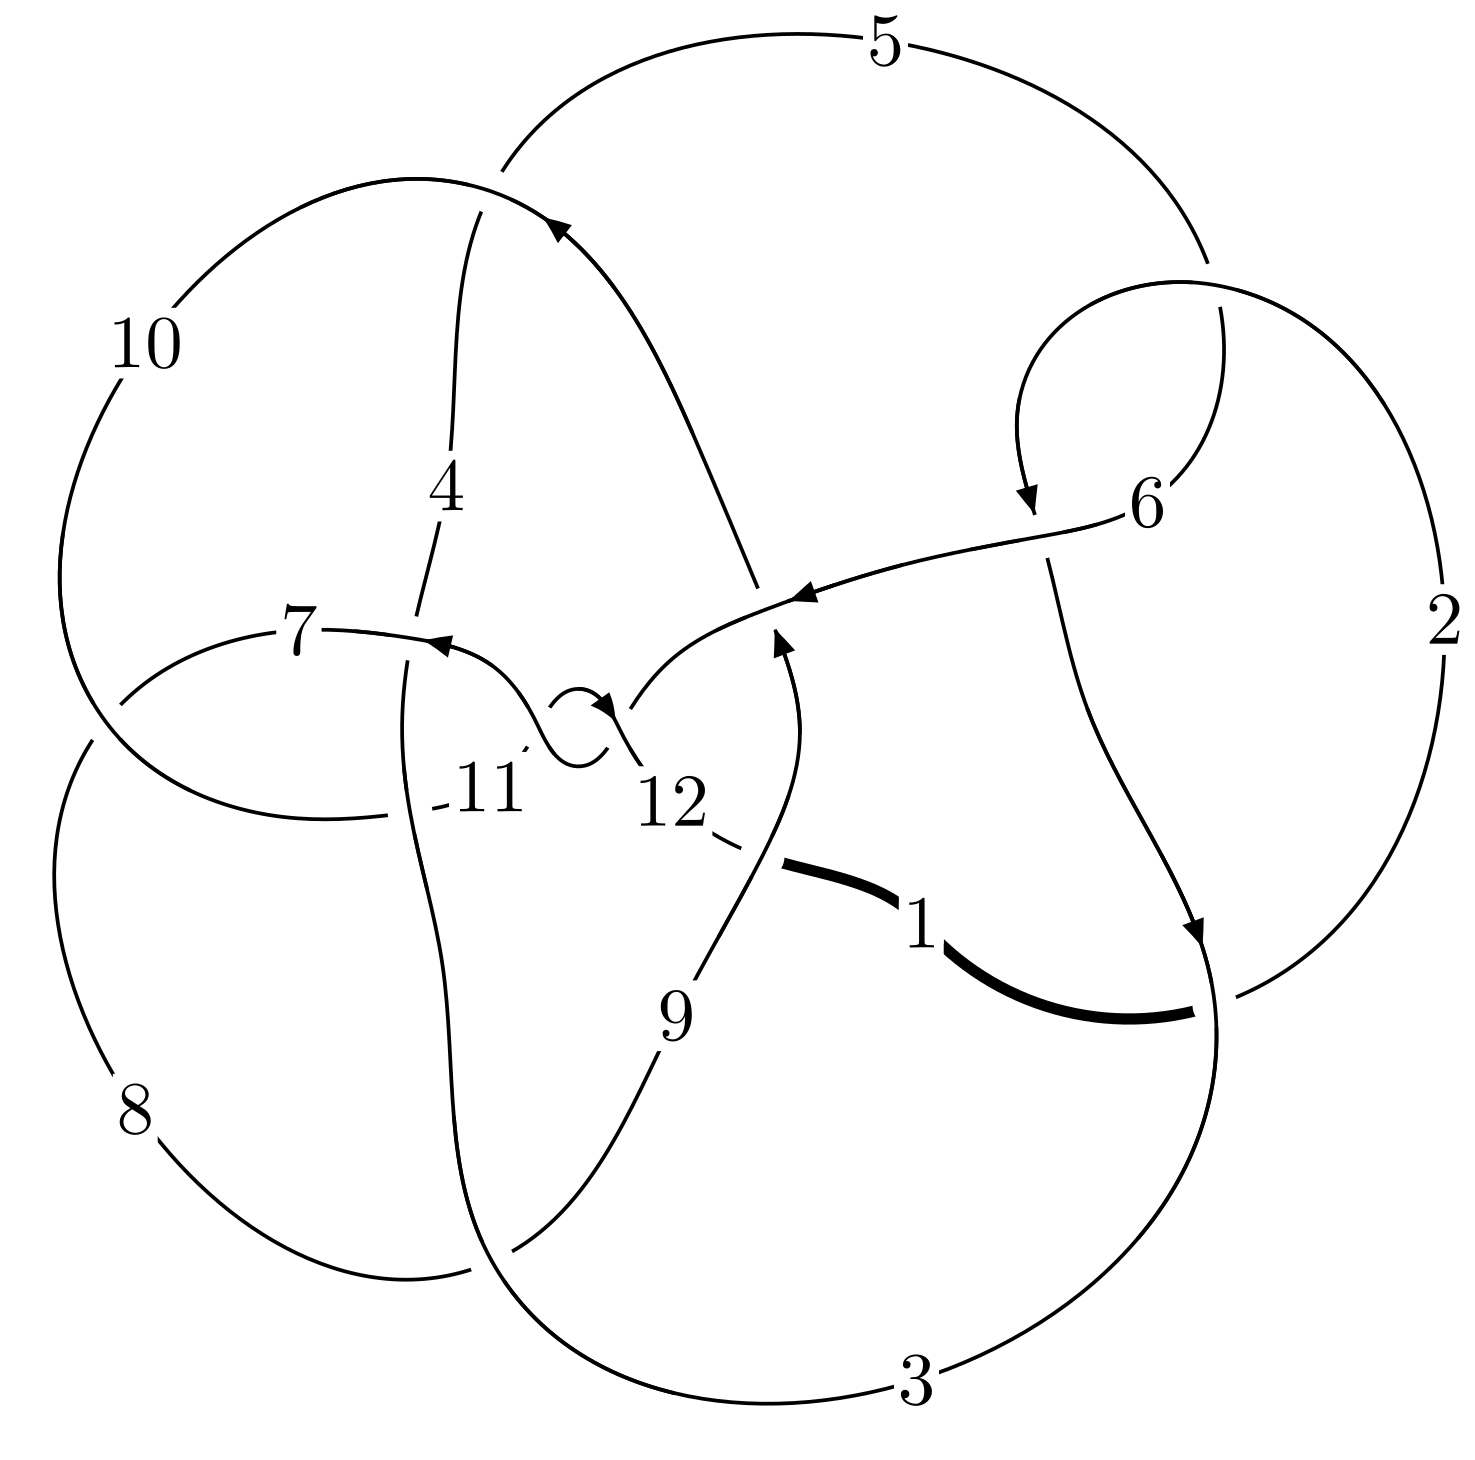
\includegraphics[width=112pt]{../../../GIT/diagram.site/Diagrams/png/2540_12n_0451.png}\\
\ \ \ A knot diagram\footnotemark}&
\allowdisplaybreaks
\textbf{Linearized knot diagam} \\
\cline{2-2}
 &
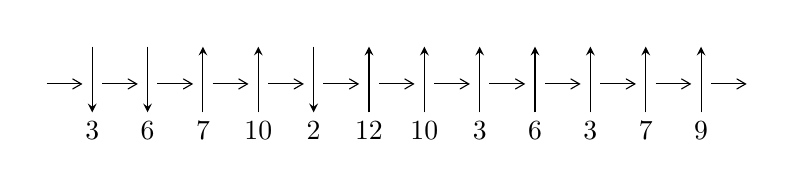
\begin{tikzpicture}[x=20pt, y=17pt]
	% nodes
	\node (C0) at (0, 0) {};
	\node (C1) at (1, 0) {};
	\node (C1U) at (1, +1) {};
	\node (C1D) at (1, -1) {3};

	\node (C2) at (2, 0) {};
	\node (C2U) at (2, +1) {};
	\node (C2D) at (2, -1) {6};

	\node (C3) at (3, 0) {};
	\node (C3U) at (3, +1) {};
	\node (C3D) at (3, -1) {7};

	\node (C4) at (4, 0) {};
	\node (C4U) at (4, +1) {};
	\node (C4D) at (4, -1) {10};

	\node (C5) at (5, 0) {};
	\node (C5U) at (5, +1) {};
	\node (C5D) at (5, -1) {2};

	\node (C6) at (6, 0) {};
	\node (C6U) at (6, +1) {};
	\node (C6D) at (6, -1) {12};

	\node (C7) at (7, 0) {};
	\node (C7U) at (7, +1) {};
	\node (C7D) at (7, -1) {10};

	\node (C8) at (8, 0) {};
	\node (C8U) at (8, +1) {};
	\node (C8D) at (8, -1) {3};

	\node (C9) at (9, 0) {};
	\node (C9U) at (9, +1) {};
	\node (C9D) at (9, -1) {6};

	\node (C10) at (10, 0) {};
	\node (C10U) at (10, +1) {};
	\node (C10D) at (10, -1) {3};

	\node (C11) at (11, 0) {};
	\node (C11U) at (11, +1) {};
	\node (C11D) at (11, -1) {7};

	\node (C12) at (12, 0) {};
	\node (C12U) at (12, +1) {};
	\node (C12D) at (12, -1) {9};
	\node (C13) at (13, 0) {};

	% arrows
	\draw[->,>={angle 60}]
	(C0) edge (C1) (C1) edge (C2) (C2) edge (C3) (C3) edge (C4) (C4) edge (C5) (C5) edge (C6) (C6) edge (C7) (C7) edge (C8) (C8) edge (C9) (C9) edge (C10) (C10) edge (C11) (C11) edge (C12) (C12) edge (C13) ;	\draw[->,>=stealth]
	(C1U) edge (C1D) (C2U) edge (C2D) (C3D) edge (C3U) (C4D) edge (C4U) (C5U) edge (C5D) (C6D) edge (C6U) (C7D) edge (C7U) (C8D) edge (C8U) (C9D) edge (C9U) (C10D) edge (C10U) (C11D) edge (C11U) (C12D) edge (C12U) ;
	\end{tikzpicture} \\
\hhline{~~} \\& 
\textbf{Solving Sequence} \\ \cline{2-2} 
 &
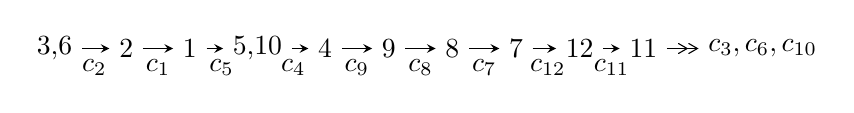
\begin{tikzpicture}[x=23pt, y=7pt]
	% node
	\node (A0) at (-1/8, 0) {3,6};
	\node (A1) at (1, 0) {2};
	\node (A2) at (2, 0) {1};
	\node (A3) at (49/16, 0) {5,10};
	\node (A4) at (33/8, 0) {4};
	\node (A5) at (41/8, 0) {9};
	\node (A6) at (49/8, 0) {8};
	\node (A7) at (57/8, 0) {7};
	\node (A8) at (65/8, 0) {12};
	\node (A9) at (73/8, 0) {11};
	\node (C1) at (1/2, -1) {$c_{2}$};
	\node (C2) at (3/2, -1) {$c_{1}$};
	\node (C3) at (5/2, -1) {$c_{5}$};
	\node (C4) at (29/8, -1) {$c_{4}$};
	\node (C5) at (37/8, -1) {$c_{9}$};
	\node (C6) at (45/8, -1) {$c_{8}$};
	\node (C7) at (53/8, -1) {$c_{7}$};
	\node (C8) at (61/8, -1) {$c_{12}$};
	\node (C9) at (69/8, -1) {$c_{11}$};
	\node (A10) at (11, 0) {$c_{3},c_{6},c_{10}$};

	% edge
	\draw[->,>=stealth]	
	(A0) edge (A1) (A1) edge (A2) (A2) edge (A3) (A3) edge (A4) (A4) edge (A5) (A5) edge (A6) (A6) edge (A7) (A7) edge (A8) (A8) edge (A9) ;
	\draw[->>,>={angle 60}]	
	(A9) edge (A10);
\end{tikzpicture} \\ 

\end{tabular} \\

\footnotetext{
The image of knot diagram is generated by the software ``\textbf{Draw programme}" developed by Andrew Bartholomew(\url{http://www.layer8.co.uk/maths/draw/index.htm\#Running-draw}), where we modified some parts for our purpose(\url{https://github.com/CATsTAILs/LinksPainter}).
}\phantom \\ \newline 
\centering \textbf{Ideals for irreducible components\footnotemark of $X_{\text{par}}$} 
 
\begin{align*}
I^u_{1}&=\langle 
13 u^{14}-82 u^{13}+\cdots+2 b-28,\;- u^{14}+3 u^{13}+\cdots+2 a+7,\;u^{15}-8 u^{14}+\cdots+18 u+4\rangle \\
I^u_{2}&=\langle 
- u^7- u^6+4 u^5+3 u^4-5 u^3-3 u^2+b+2 u+1,\\
\phantom{I^u_{2}}&\phantom{= \langle  }2 u^9+6 u^8- u^7-18 u^6-10 u^5+18 u^4+15 u^3-4 u^2+3 a-4 u+1,\\
\phantom{I^u_{2}}&\phantom{= \langle  }u^{10}+3 u^9-2 u^8-12 u^7-2 u^6+18 u^5+9 u^4-11 u^3-8 u^2+2 u+3\rangle \\
I^u_{3}&=\langle 
a^3 u^2+8 a^3 u+6 a^2 u^2+2 a^3+9 a^2 u- a^2-3 u^2+13 b-11 u-6,\\
\phantom{I^u_{3}}&\phantom{= \langle  }-2 a^3 u^2+a^4- a^3 u-3 a^2 u^2+4 a^3-3 a^2 u-6 u^2 a+7 a^2-3 a u-16 u^2+13 a-9 u+37,\;u^3+u^2-2 u-1\rangle \\
\\
\end{align*}
\raggedright * 3 irreducible components of $\dim_{\mathbb{C}}=0$, with total 37 representations.\\
\footnotetext{All coefficients of polynomials are rational numbers. But the coefficients are sometimes approximated in decimal forms when there is not enough margin.}
\newpage
\renewcommand{\arraystretch}{1}
\centering \section*{I. $I^u_{1}= \langle 13 u^{14}-82 u^{13}+\cdots+2 b-28,\;- u^{14}+3 u^{13}+\cdots+2 a+7,\;u^{15}-8 u^{14}+\cdots+18 u+4 \rangle$}
\flushleft \textbf{(i) Arc colorings}\\
\begin{tabular}{m{7pt} m{180pt} m{7pt} m{180pt} }
\flushright $a_{3}=$&$\begin{pmatrix}1\\0\end{pmatrix}$ \\
\flushright $a_{6}=$&$\begin{pmatrix}0\\u\end{pmatrix}$ \\
\flushright $a_{2}=$&$\begin{pmatrix}1\\- u^2\end{pmatrix}$ \\
\flushright $a_{1}=$&$\begin{pmatrix}- u^2+1\\- u^2\end{pmatrix}$ \\
\flushright $a_{5}=$&$\begin{pmatrix}u\\- u^3+u\end{pmatrix}$ \\
\flushright $a_{10}=$&$\begin{pmatrix}\frac{1}{2} u^{14}-\frac{3}{2} u^{13}+\cdots-\frac{3}{2} u-\frac{7}{2}\\-\frac{13}{2} u^{14}+41 u^{13}+\cdots+\frac{145}{2} u+14\end{pmatrix}$ \\
\flushright $a_{4}=$&$\begin{pmatrix}\frac{19}{4} u^{14}-\frac{61}{2} u^{13}+\cdots-\frac{239}{4} u-11\\\frac{1}{2} u^{14}-3 u^{13}+\cdots-\frac{9}{2} u-1\end{pmatrix}$ \\
\flushright $a_{9}=$&$\begin{pmatrix}\frac{1}{2} u^{14}-\frac{3}{2} u^{13}+\cdots-\frac{3}{2} u-\frac{7}{2}\\-\frac{1}{2} u^{14}+6 u^{13}+\cdots+\frac{51}{2} u+4\end{pmatrix}$ \\
\flushright $a_{8}=$&$\begin{pmatrix}u^{14}-\frac{15}{2} u^{13}+\cdots-27 u-\frac{15}{2}\\-\frac{1}{2} u^{14}+6 u^{13}+\cdots+\frac{51}{2} u+4\end{pmatrix}$ \\
\flushright $a_{7}=$&$\begin{pmatrix}-\frac{1}{2} u^{14}+\frac{7}{2} u^{13}+\cdots-\frac{3}{2} u-\frac{3}{2}\\-\frac{13}{2} u^{14}+41 u^{13}+\cdots+\frac{145}{2} u+14\end{pmatrix}$ \\
\flushright $a_{12}=$&$\begin{pmatrix}-\frac{11}{4} u^{14}+\frac{35}{2} u^{13}+\cdots+\frac{143}{4} u+9\\-\frac{15}{2} u^{14}+48 u^{13}+\cdots+\frac{193}{2} u+19\end{pmatrix}$ \\
\flushright $a_{11}=$&$\begin{pmatrix}6 u^{14}-\frac{79}{2} u^{13}+\cdots-71 u-\frac{21}{2}\\\frac{13}{2} u^{14}-41 u^{13}+\cdots-\frac{145}{2} u-14\end{pmatrix}$\\&\end{tabular}
\flushleft \textbf{(ii) Obstruction class $= -1$}\\~\\
\flushleft \textbf{(iii) Cusp Shapes $= -14 u^{14}+88 u^{13}-169 u^{12}+49 u^{11}+u^{10}+512 u^9-618 u^8-173 u^7-82 u^6+878 u^5-86 u^4-524 u^3-44 u^2+156 u+46$}\\~\\
\newpage\renewcommand{\arraystretch}{1}
\flushleft \textbf{(iv) u-Polynomials at the component}\newline \\
\begin{tabular}{m{50pt}|m{274pt}}
Crossings & \hspace{64pt}u-Polynomials at each crossing \\
\hline $$\begin{aligned}c_{1}\end{aligned}$$&$\begin{aligned}
&u^{15}+18 u^{14}+\cdots+428 u+16
\end{aligned}$\\
\hline $$\begin{aligned}c_{2},c_{5}\end{aligned}$$&$\begin{aligned}
&u^{15}+8 u^{14}+\cdots+18 u-4
\end{aligned}$\\
\hline $$\begin{aligned}c_{3},c_{10}\end{aligned}$$&$\begin{aligned}
&u^{15}- u^{14}+\cdots- u-1
\end{aligned}$\\
\hline $$\begin{aligned}c_{4},c_{8}\end{aligned}$$&$\begin{aligned}
&u^{15}+15 u^{13}+\cdots-5 u^2-1
\end{aligned}$\\
\hline $$\begin{aligned}c_{6},c_{11}\end{aligned}$$&$\begin{aligned}
&u^{15}-8 u^{14}+\cdots+44 u-8
\end{aligned}$\\
\hline $$\begin{aligned}c_{7}\end{aligned}$$&$\begin{aligned}
&u^{15}+11 u^{14}+\cdots-30 u-4
\end{aligned}$\\
\hline $$\begin{aligned}c_{9},c_{12}\end{aligned}$$&$\begin{aligned}
&u^{15}+u^{14}+\cdots-10 u-1
\end{aligned}$\\
\hline
\end{tabular}\\~\\
\newpage\renewcommand{\arraystretch}{1}
\flushleft \textbf{(v) Riley Polynomials at the component}\newline \\
\begin{tabular}{m{50pt}|m{274pt}}
Crossings & \hspace{64pt}Riley Polynomials at each crossing \\
\hline $$\begin{aligned}c_{1}\end{aligned}$$&$\begin{aligned}
&y^{15}-38 y^{14}+\cdots+98672 y-256
\end{aligned}$\\
\hline $$\begin{aligned}c_{2},c_{5}\end{aligned}$$&$\begin{aligned}
&y^{15}-18 y^{14}+\cdots+428 y-16
\end{aligned}$\\
\hline $$\begin{aligned}c_{3},c_{10}\end{aligned}$$&$\begin{aligned}
&y^{15}-19 y^{14}+\cdots+23 y-1
\end{aligned}$\\
\hline $$\begin{aligned}c_{4},c_{8}\end{aligned}$$&$\begin{aligned}
&y^{15}+30 y^{14}+\cdots-10 y-1
\end{aligned}$\\
\hline $$\begin{aligned}c_{6},c_{11}\end{aligned}$$&$\begin{aligned}
&y^{15}+8 y^{14}+\cdots+144 y-64
\end{aligned}$\\
\hline $$\begin{aligned}c_{7}\end{aligned}$$&$\begin{aligned}
&y^{15}+5 y^{14}+\cdots+108 y-16
\end{aligned}$\\
\hline $$\begin{aligned}c_{9},c_{12}\end{aligned}$$&$\begin{aligned}
&y^{15}+19 y^{14}+\cdots+54 y-1
\end{aligned}$\\
\hline
\end{tabular}\\~\\
\newpage\flushleft \textbf{(vi) Complex Volumes and Cusp Shapes}
$$\begin{array}{c|c|c}  
\text{Solutions to }I^u_{1}& \I (\text{vol} + \sqrt{-1}CS) & \text{Cusp shape}\\
 \hline 
\begin{aligned}
u &= \phantom{-}0.959509 + 0.354430 I \\
a &= -0.161134 + 0.086188 I \\
b &= \phantom{-}0.316905 + 0.548611 I\end{aligned}
 & -1.65521 - 1.25769 I & \phantom{-}0.52360 + 4.10357 I \\ \hline\begin{aligned}
u &= \phantom{-}0.959509 - 0.354430 I \\
a &= -0.161134 - 0.086188 I \\
b &= \phantom{-}0.316905 - 0.548611 I\end{aligned}
 & -1.65521 + 1.25769 I & \phantom{-}0.52360 - 4.10357 I \\ \hline\begin{aligned}
u &= -0.550498 + 0.994483 I \\
a &= -0.718395 + 0.573199 I \\
b &= -1.342500 + 0.128424 I\end{aligned}
 & \phantom{-}2.97662 - 0.13213 I & \phantom{-}5.02719 - 0.29116 I \\ \hline\begin{aligned}
u &= -0.550498 - 0.994483 I \\
a &= -0.718395 - 0.573199 I \\
b &= -1.342500 - 0.128424 I\end{aligned}
 & \phantom{-}2.97662 + 0.13213 I & \phantom{-}5.02719 + 0.29116 I \\ \hline\begin{aligned}
u &= -0.946416 + 0.902266 I \\
a &= \phantom{-}0.592748 - 0.766485 I \\
b &= \phantom{-}1.45247 + 0.51633 I\end{aligned}
 & \phantom{-}1.73111 + 6.58453 I & \phantom{-}3.78417 - 5.80099 I \\ \hline\begin{aligned}
u &= -0.946416 - 0.902266 I \\
a &= \phantom{-}0.592748 + 0.766485 I \\
b &= \phantom{-}1.45247 - 0.51633 I\end{aligned}
 & \phantom{-}1.73111 - 6.58453 I & \phantom{-}3.78417 + 5.80099 I \\ \hline\begin{aligned}
u &= -0.484300 + 0.231140 I \\
a &= \phantom{-}1.92354 - 0.88468 I \\
b &= \phantom{-}0.417351 + 0.091087 I\end{aligned}
 & -3.75387 - 2.45110 I & \phantom{-}11.17942 + 2.61787 I \\ \hline\begin{aligned}
u &= -0.484300 - 0.231140 I \\
a &= \phantom{-}1.92354 + 0.88468 I \\
b &= \phantom{-}0.417351 - 0.091087 I\end{aligned}
 & -3.75387 + 2.45110 I & \phantom{-}11.17942 - 2.61787 I \\ \hline\begin{aligned}
u &= \phantom{-}1.61285 + 0.22347 I \\
a &= -0.112650 - 0.865027 I \\
b &= -1.065320 + 0.236511 I\end{aligned}
 & -10.89750 + 0.20978 I & \phantom{-}2.15059 - 0.10319 I \\ \hline\begin{aligned}
u &= \phantom{-}1.61285 - 0.22347 I \\
a &= -0.112650 + 0.865027 I \\
b &= -1.065320 - 0.236511 I\end{aligned}
 & -10.89750 - 0.20978 I & \phantom{-}2.15059 + 0.10319 I\\
 \hline 
 \end{array}$$\newpage$$\begin{array}{c|c|c}  
\text{Solutions to }I^u_{1}& \I (\text{vol} + \sqrt{-1}CS) & \text{Cusp shape}\\
 \hline 
\begin{aligned}
u &= \phantom{-}1.72721 + 0.30285 I \\
a &= -0.232010 + 0.919021 I \\
b &= \phantom{-}1.57691 - 0.30542 I\end{aligned}
 & -4.83321 - 4.76833 I & \phantom{-}4.97369 + 2.14836 I \\ \hline\begin{aligned}
u &= \phantom{-}1.72721 - 0.30285 I \\
a &= -0.232010 - 0.919021 I \\
b &= \phantom{-}1.57691 + 0.30542 I\end{aligned}
 & -4.83321 + 4.76833 I & \phantom{-}4.97369 - 2.14836 I \\ \hline\begin{aligned}
u &= -0.224907\phantom{ +0.000000I} \\
a &= -2.25152\phantom{ +0.000000I} \\
b &= -0.299515\phantom{ +0.000000I}\end{aligned}
 & \phantom{-}0.730621\phantom{ +0.000000I} & \phantom{-}13.9140\phantom{ +0.000000I} \\ \hline\begin{aligned}
u &= \phantom{-}1.79410 + 0.24246 I \\
a &= \phantom{-}0.333662 - 1.121120 I \\
b &= -1.70606 + 0.72255 I\end{aligned}
 & -7.78478 - 11.23000 I & \phantom{-}2.90412 + 5.28147 I \\ \hline\begin{aligned}
u &= \phantom{-}1.79410 - 0.24246 I \\
a &= \phantom{-}0.333662 + 1.121120 I \\
b &= -1.70606 - 0.72255 I\end{aligned}
 & -7.78478 + 11.23000 I & \phantom{-}2.90412 - 5.28147 I\\
 \hline 
 \end{array}$$\newpage\newpage\renewcommand{\arraystretch}{1}
\centering \section*{II. $I^u_{2}= \langle - u^7- u^6+\cdots+b+1,\;2 u^9+6 u^8+\cdots+3 a+1,\;u^{10}+3 u^9+\cdots+2 u+3 \rangle$}
\flushleft \textbf{(i) Arc colorings}\\
\begin{tabular}{m{7pt} m{180pt} m{7pt} m{180pt} }
\flushright $a_{3}=$&$\begin{pmatrix}1\\0\end{pmatrix}$ \\
\flushright $a_{6}=$&$\begin{pmatrix}0\\u\end{pmatrix}$ \\
\flushright $a_{2}=$&$\begin{pmatrix}1\\- u^2\end{pmatrix}$ \\
\flushright $a_{1}=$&$\begin{pmatrix}- u^2+1\\- u^2\end{pmatrix}$ \\
\flushright $a_{5}=$&$\begin{pmatrix}u\\- u^3+u\end{pmatrix}$ \\
\flushright $a_{10}=$&$\begin{pmatrix}-\frac{2}{3} u^9-2 u^8+\cdots+\frac{4}{3} u-\frac{1}{3}\\u^7+u^6-4 u^5-3 u^4+5 u^3+3 u^2-2 u-1\end{pmatrix}$ \\
\flushright $a_{4}=$&$\begin{pmatrix}\frac{1}{3} u^9-\frac{8}{3} u^7+\cdots+\frac{7}{3} u+\frac{8}{3}\\- u^3+2 u-1\end{pmatrix}$ \\
\flushright $a_{9}=$&$\begin{pmatrix}-\frac{2}{3} u^9-2 u^8+\cdots+\frac{4}{3} u-\frac{1}{3}\\- u^9-2 u^8+3 u^7+7 u^6-3 u^5-9 u^4+u^3+4 u^2-1\end{pmatrix}$ \\
\flushright $a_{8}=$&$\begin{pmatrix}\frac{1}{3} u^9-\frac{8}{3} u^7+\cdots+\frac{4}{3} u+\frac{2}{3}\\- u^9-2 u^8+3 u^7+7 u^6-3 u^5-9 u^4+u^3+4 u^2-1\end{pmatrix}$ \\
\flushright $a_{7}=$&$\begin{pmatrix}\frac{2}{3} u^9+2 u^8+\cdots-\frac{10}{3} u-\frac{2}{3}\\- u^7- u^6+4 u^5+3 u^4-5 u^3-3 u^2+2 u+1\end{pmatrix}$ \\
\flushright $a_{12}=$&$\begin{pmatrix}\frac{2}{3} u^9+2 u^8+\cdots-\frac{10}{3} u-\frac{2}{3}\\u^9+2 u^8-3 u^7-7 u^6+2 u^5+9 u^4+2 u^3-5 u^2-2 u+1\end{pmatrix}$ \\
\flushright $a_{11}=$&$\begin{pmatrix}-\frac{2}{3} u^9-2 u^8+\cdots-\frac{2}{3} u-\frac{4}{3}\\u^7+u^6-4 u^5-3 u^4+5 u^3+3 u^2-2 u-1\end{pmatrix}$\\&\end{tabular}
\flushleft \textbf{(ii) Obstruction class $= 1$}\\~\\
\flushleft \textbf{(iii) Cusp Shapes $= -3 u^9-8 u^8+5 u^7+23 u^6+u^5-21 u^4-5 u^3+3 u^2-4 u+3$}\\~\\
\newpage\renewcommand{\arraystretch}{1}
\flushleft \textbf{(iv) u-Polynomials at the component}\newline \\
\begin{tabular}{m{50pt}|m{274pt}}
Crossings & \hspace{64pt}u-Polynomials at each crossing \\
\hline $$\begin{aligned}c_{1}\end{aligned}$$&$\begin{aligned}
&u^{10}-13 u^9+\cdots-52 u+9
\end{aligned}$\\
\hline $$\begin{aligned}c_{2}\end{aligned}$$&$\begin{aligned}
&u^{10}+3 u^9-2 u^8-12 u^7-2 u^6+18 u^5+9 u^4-11 u^3-8 u^2+2 u+3
\end{aligned}$\\
\hline $$\begin{aligned}c_{3},c_{10}\end{aligned}$$&$\begin{aligned}
&u^{10}- u^9-3 u^8+3 u^7- u^6+2 u^5+5 u^4-9 u^3+7 u^2-2 u+1
\end{aligned}$\\
\hline $$\begin{aligned}c_{4},c_{8}\end{aligned}$$&$\begin{aligned}
&u^{10}+3 u^8-4 u^7-11 u^6+11 u^5+13 u^4-6 u^3-2 u^2+3 u+1
\end{aligned}$\\
\hline $$\begin{aligned}c_{5}\end{aligned}$$&$\begin{aligned}
&u^{10}-3 u^9-2 u^8+12 u^7-2 u^6-18 u^5+9 u^4+11 u^3-8 u^2-2 u+3
\end{aligned}$\\
\hline $$\begin{aligned}c_{6}\end{aligned}$$&$\begin{aligned}
&u^{10}- u^9+4 u^8-3 u^7+7 u^6-3 u^5+5 u^4- u^3+2 u^2+u+1
\end{aligned}$\\
\hline $$\begin{aligned}c_{7}\end{aligned}$$&$\begin{aligned}
&u^{10}+6 u^9+13 u^8+12 u^7+5 u^6+2 u^5+4 u^4+22 u^3+41 u^2+28 u+7
\end{aligned}$\\
\hline $$\begin{aligned}c_{9},c_{12}\end{aligned}$$&$\begin{aligned}
&u^{10}- u^9+4 u^8-6 u^7+4 u^6-6 u^5+10 u^4-9 u^3+6 u^2-3 u+1
\end{aligned}$\\
\hline $$\begin{aligned}c_{11}\end{aligned}$$&$\begin{aligned}
&u^{10}+u^9+4 u^8+3 u^7+7 u^6+3 u^5+5 u^4+u^3+2 u^2- u+1
\end{aligned}$\\
\hline
\end{tabular}\\~\\
\newpage\renewcommand{\arraystretch}{1}
\flushleft \textbf{(v) Riley Polynomials at the component}\newline \\
\begin{tabular}{m{50pt}|m{274pt}}
Crossings & \hspace{64pt}Riley Polynomials at each crossing \\
\hline $$\begin{aligned}c_{1}\end{aligned}$$&$\begin{aligned}
&y^{10}-25 y^9+\cdots+212 y+81
\end{aligned}$\\
\hline $$\begin{aligned}c_{2},c_{5}\end{aligned}$$&$\begin{aligned}
&y^{10}-13 y^9+\cdots-52 y+9
\end{aligned}$\\
\hline $$\begin{aligned}c_{3},c_{10}\end{aligned}$$&$\begin{aligned}
&y^{10}-7 y^9+13 y^8+11 y^7-45 y^6-4 y^5+53 y^4-5 y^3+23 y^2+10 y+1
\end{aligned}$\\
\hline $$\begin{aligned}c_{4},c_{8}\end{aligned}$$&$\begin{aligned}
&y^{10}+6 y^9+\cdots-13 y+1
\end{aligned}$\\
\hline $$\begin{aligned}c_{6},c_{11}\end{aligned}$$&$\begin{aligned}
&y^{10}+7 y^9+\cdots+3 y+1
\end{aligned}$\\
\hline $$\begin{aligned}c_{7}\end{aligned}$$&$\begin{aligned}
&y^{10}-10 y^9+\cdots-210 y+49
\end{aligned}$\\
\hline $$\begin{aligned}c_{9},c_{12}\end{aligned}$$&$\begin{aligned}
&y^{10}+7 y^9+12 y^8+4 y^7+18 y^6-20 y^5+12 y^4+11 y^3+2 y^2+3 y+1
\end{aligned}$\\
\hline
\end{tabular}\\~\\
\newpage\flushleft \textbf{(vi) Complex Volumes and Cusp Shapes}
$$\begin{array}{c|c|c}  
\text{Solutions to }I^u_{2}& \I (\text{vol} + \sqrt{-1}CS) & \text{Cusp shape}\\
 \hline 
\begin{aligned}
u &= \phantom{-}0.794660 + 0.197895 I \\
a &= -1.21999 - 0.81881 I \\
b &= -0.033564 + 0.426607 I\end{aligned}
 & -4.30076 + 2.46712 I & -4.14664 - 2.94515 I \\ \hline\begin{aligned}
u &= \phantom{-}0.794660 - 0.197895 I \\
a &= -1.21999 + 0.81881 I \\
b &= -0.033564 - 0.426607 I\end{aligned}
 & -4.30076 - 2.46712 I & -4.14664 + 2.94515 I \\ \hline\begin{aligned}
u &= -1.154300 + 0.430931 I \\
a &= -0.174417 + 0.481835 I \\
b &= -1.57328 - 0.24809 I\end{aligned}
 & \phantom{-}3.14814 + 4.53334 I & \phantom{-}4.18402 - 3.64382 I \\ \hline\begin{aligned}
u &= -1.154300 - 0.430931 I \\
a &= -0.174417 - 0.481835 I \\
b &= -1.57328 + 0.24809 I\end{aligned}
 & \phantom{-}3.14814 - 4.53334 I & \phantom{-}4.18402 + 3.64382 I \\ \hline\begin{aligned}
u &= -0.563250 + 0.505340 I \\
a &= -0.146187 - 0.911256 I \\
b &= \phantom{-}1.55694 - 0.21156 I\end{aligned}
 & \phantom{-}5.07321 - 0.90406 I & \phantom{-}8.90897 - 1.12395 I \\ \hline\begin{aligned}
u &= -0.563250 - 0.505340 I \\
a &= -0.146187 + 0.911256 I \\
b &= \phantom{-}1.55694 + 0.21156 I\end{aligned}
 & \phantom{-}5.07321 + 0.90406 I & \phantom{-}8.90897 + 1.12395 I \\ \hline\begin{aligned}
u &= \phantom{-}1.228530 + 0.260062 I \\
a &= \phantom{-}0.760530 + 0.065247 I \\
b &= -0.634254 - 0.504382 I\end{aligned}
 & -1.184580 - 0.336842 I & \phantom{-}3.77741 - 2.24920 I \\ \hline\begin{aligned}
u &= \phantom{-}1.228530 - 0.260062 I \\
a &= \phantom{-}0.760530 - 0.065247 I \\
b &= -0.634254 + 0.504382 I\end{aligned}
 & -1.184580 + 0.336842 I & \phantom{-}3.77741 + 2.24920 I \\ \hline\begin{aligned}
u &= -1.80564 + 0.05386 I \\
a &= \phantom{-}0.113401 - 1.082570 I \\
b &= \phantom{-}0.184156 + 1.137500 I\end{aligned}
 & -14.2505 - 0.9863 I & -1.223765 + 0.251668 I \\ \hline\begin{aligned}
u &= -1.80564 - 0.05386 I \\
a &= \phantom{-}0.113401 + 1.082570 I \\
b &= \phantom{-}0.184156 - 1.137500 I\end{aligned}
 & -14.2505 + 0.9863 I & -1.223765 - 0.251668 I\\
 \hline 
 \end{array}$$\newpage\newpage\renewcommand{\arraystretch}{1}
\centering \section*{III. $I^u_{3}= \langle a^3 u^2+6 a^2 u^2+\cdots- a^2-6,\;-2 a^3 u^2-3 a^2 u^2+\cdots+13 a+37,\;u^3+u^2-2 u-1 \rangle$}
\flushleft \textbf{(i) Arc colorings}\\
\begin{tabular}{m{7pt} m{180pt} m{7pt} m{180pt} }
\flushright $a_{3}=$&$\begin{pmatrix}1\\0\end{pmatrix}$ \\
\flushright $a_{6}=$&$\begin{pmatrix}0\\u\end{pmatrix}$ \\
\flushright $a_{2}=$&$\begin{pmatrix}1\\- u^2\end{pmatrix}$ \\
\flushright $a_{1}=$&$\begin{pmatrix}- u^2+1\\- u^2\end{pmatrix}$ \\
\flushright $a_{5}=$&$\begin{pmatrix}u\\u^2- u-1\end{pmatrix}$ \\
\flushright $a_{10}=$&$\begin{pmatrix}a\\-0.0769231 a^{3} u^{2}-0.461538 a^{2} u^{2}+\cdots+0.0769231 a^{2}+0.461538\end{pmatrix}$ \\
\flushright $a_{4}=$&$\begin{pmatrix}-0.615385 a^{3} u^{2}-0.692308 a^{2} u^{2}+\cdots+a+1.69231\\\frac{8}{13} a^3 u^2+\frac{9}{13} a^2 u^2+\cdots- a-\frac{48}{13}\end{pmatrix}$ \\
\flushright $a_{9}=$&$\begin{pmatrix}a\\-0.0769231 a^{3} u^{2}-0.461538 a^{2} u^{2}+\cdots+0.0769231 a^{2}+0.461538\end{pmatrix}$ \\
\flushright $a_{8}=$&$\begin{pmatrix}\frac{1}{13} a^3 u^2+\frac{6}{13} a^2 u^2+\cdots+a-\frac{6}{13}\\-0.0769231 a^{3} u^{2}-0.461538 a^{2} u^{2}+\cdots+0.0769231 a^{2}+0.461538\end{pmatrix}$ \\
\flushright $a_{7}=$&$\begin{pmatrix}\frac{1}{13} a^3 u^2+\frac{6}{13} a^2 u^2+\cdots- a-\frac{6}{13}\\0.307692 a^{3} u^{2}-0.153846 a^{2} u^{2}+\cdots-0.307692 a^{2}+0.153846\end{pmatrix}$ \\
\flushright $a_{12}=$&$\begin{pmatrix}\frac{1}{13} a^3 u^2+\frac{6}{13} a^2 u^2+\cdots- a-\frac{32}{13}\\-0.538462 a^{3} u^{2}+0.769231 a^{2} u^{2}+\cdots-0.461538 a^{2}-0.769231\end{pmatrix}$ \\
\flushright $a_{11}=$&$\begin{pmatrix}\frac{1}{13} a^3 u^2+\frac{6}{13} a^2 u^2+\cdots- a-\frac{6}{13}\\0.0769231 a^{3} u^{2}+0.461538 a^{2} u^{2}+\cdots-0.0769231 a^{2}-0.461538\end{pmatrix}$\\&\end{tabular}
\flushleft \textbf{(ii) Obstruction class $= -1$}\\~\\
\flushleft \textbf{(iii) Cusp Shapes $= -\frac{28}{13} a^3 u^2-\frac{16}{13} a^3 u-\frac{12}{13} a^2 u^2-\frac{4}{13} a^3-\frac{44}{13} a^2 u-\frac{24}{13} a^2+4 a u+\frac{32}{13} u^2+\frac{48}{13} u+\frac{38}{13}$}\\~\\
\newpage\renewcommand{\arraystretch}{1}
\flushleft \textbf{(iv) u-Polynomials at the component}\newline \\
\begin{tabular}{m{50pt}|m{274pt}}
Crossings & \hspace{64pt}u-Polynomials at each crossing \\
\hline $$\begin{aligned}c_{1}\end{aligned}$$&$\begin{aligned}
&(u^3+5 u^2+6 u+1)^4
\end{aligned}$\\
\hline $$\begin{aligned}c_{2},c_{5},c_{7}\end{aligned}$$&$\begin{aligned}
&(u^3- u^2-2 u+1)^4
\end{aligned}$\\
\hline $$\begin{aligned}c_{3},c_{10}\end{aligned}$$&$\begin{aligned}
&u^{12}- u^{11}+\cdots-34 u+13
\end{aligned}$\\
\hline $$\begin{aligned}c_{4},c_{8}\end{aligned}$$&$\begin{aligned}
&u^{12}+u^{11}+\cdots+208 u+139
\end{aligned}$\\
\hline $$\begin{aligned}c_{6},c_{11}\end{aligned}$$&$\begin{aligned}
&(u^2+u+1)^6
\end{aligned}$\\
\hline $$\begin{aligned}c_{9},c_{12}\end{aligned}$$&$\begin{aligned}
&u^{12}- u^{11}+\cdots-16 u+43
\end{aligned}$\\
\hline
\end{tabular}\\~\\
\newpage\renewcommand{\arraystretch}{1}
\flushleft \textbf{(v) Riley Polynomials at the component}\newline \\
\begin{tabular}{m{50pt}|m{274pt}}
Crossings & \hspace{64pt}Riley Polynomials at each crossing \\
\hline $$\begin{aligned}c_{1}\end{aligned}$$&$\begin{aligned}
&(y^3-13 y^2+26 y-1)^4
\end{aligned}$\\
\hline $$\begin{aligned}c_{2},c_{5},c_{7}\end{aligned}$$&$\begin{aligned}
&(y^3-5 y^2+6 y-1)^4
\end{aligned}$\\
\hline $$\begin{aligned}c_{3},c_{10}\end{aligned}$$&$\begin{aligned}
&y^{12}-5 y^{11}+\cdots-740 y+169
\end{aligned}$\\
\hline $$\begin{aligned}c_{4},c_{8}\end{aligned}$$&$\begin{aligned}
&y^{12}+19 y^{11}+\cdots+24568 y+19321
\end{aligned}$\\
\hline $$\begin{aligned}c_{6},c_{11}\end{aligned}$$&$\begin{aligned}
&(y^2+y+1)^6
\end{aligned}$\\
\hline $$\begin{aligned}c_{9},c_{12}\end{aligned}$$&$\begin{aligned}
&y^{12}+11 y^{11}+\cdots+948 y+1849
\end{aligned}$\\
\hline
\end{tabular}\\~\\
\newpage\flushleft \textbf{(vi) Complex Volumes and Cusp Shapes}
$$\begin{array}{c|c|c}  
\text{Solutions to }I^u_{3}& \I (\text{vol} + \sqrt{-1}CS) & \text{Cusp shape}\\
 \hline 
\begin{aligned}
u &= \phantom{-}1.24698\phantom{ +0.000000I} \\
a &= \phantom{-}1.002800 + 0.135184 I \\
b &= -0.601826 - 0.829682 I\end{aligned}
 & -1.40994 + 2.02988 I & \phantom{-}4.00000 - 3.46410 I \\ \hline\begin{aligned}
u &= \phantom{-}1.24698\phantom{ +0.000000I} \\
a &= \phantom{-}1.002800 - 0.135184 I \\
b &= -0.601826 + 0.829682 I\end{aligned}
 & -1.40994 - 2.02988 I & \phantom{-}4.00000 + 3.46410 I \\ \hline\begin{aligned}
u &= \phantom{-}1.24698\phantom{ +0.000000I} \\
a &= -0.824347 + 0.444265 I \\
b &= \phantom{-}1.225320 + 0.250234 I\end{aligned}
 & -1.40994 - 2.02988 I & \phantom{-}4.00000 + 3.46410 I \\ \hline\begin{aligned}
u &= \phantom{-}1.24698\phantom{ +0.000000I} \\
a &= -0.824347 - 0.444265 I \\
b &= \phantom{-}1.225320 - 0.250234 I\end{aligned}
 & -1.40994 + 2.02988 I & \phantom{-}4.00000 - 3.46410 I \\ \hline\begin{aligned}
u &= -0.445042\phantom{ +0.000000I} \\
a &= \phantom{-}0.52051 + 2.02175 I \\
b &= -1.64400 - 0.07581 I\end{aligned}
 & \phantom{-}4.22983 + 2.02988 I & \phantom{-}4.00000 - 3.46410 I \\ \hline\begin{aligned}
u &= -0.445042\phantom{ +0.000000I} \\
a &= \phantom{-}0.52051 - 2.02175 I \\
b &= -1.64400 + 0.07581 I\end{aligned}
 & \phantom{-}4.22983 - 2.02988 I & \phantom{-}4.00000 + 3.46410 I \\ \hline\begin{aligned}
u &= -0.445042\phantom{ +0.000000I} \\
a &= -2.54497 + 1.48471 I \\
b &= \phantom{-}1.42148 + 0.46123 I\end{aligned}
 & \phantom{-}4.22983 + 2.02988 I & \phantom{-}4.00000 - 3.46410 I \\ \hline\begin{aligned}
u &= -0.445042\phantom{ +0.000000I} \\
a &= -2.54497 - 1.48471 I \\
b &= \phantom{-}1.42148 - 0.46123 I\end{aligned}
 & \phantom{-}4.22983 - 2.02988 I & \phantom{-}4.00000 + 3.46410 I \\ \hline\begin{aligned}
u &= -1.80194\phantom{ +0.000000I} \\
a &= \phantom{-}0.248738 + 0.776723 I \\
b &= -0.526217 - 0.296115 I\end{aligned}
 & -12.68950 + 2.02988 I & \phantom{-}4.00000 - 3.46410 I \\ \hline\begin{aligned}
u &= -1.80194\phantom{ +0.000000I} \\
a &= \phantom{-}0.248738 - 0.776723 I \\
b &= -0.526217 + 0.296115 I\end{aligned}
 & -12.68950 - 2.02988 I & \phantom{-}4.00000 + 3.46410 I\\
 \hline 
 \end{array}$$\newpage$$\begin{array}{c|c|c}  
\text{Solutions to }I^u_{3}& \I (\text{vol} + \sqrt{-1}CS) & \text{Cusp shape}\\
 \hline 
\begin{aligned}
u &= -1.80194\phantom{ +0.000000I} \\
a &= \phantom{-}0.097273 + 1.376030 I \\
b &= -0.37475 - 1.85664 I\end{aligned}
 & -12.68950 - 2.02988 I & \phantom{-}4.00000 + 3.46410 I \\ \hline\begin{aligned}
u &= -1.80194\phantom{ +0.000000I} \\
a &= \phantom{-}0.097273 - 1.376030 I \\
b &= -0.37475 + 1.85664 I\end{aligned}
 & -12.68950 + 2.02988 I & \phantom{-}4.00000 - 3.46410 I\\
 \hline 
 \end{array}$$\newpage
\newpage\renewcommand{\arraystretch}{1}
\centering \section*{ IV. u-Polynomials}
\begin{tabular}{m{50pt}|m{274pt}}
Crossings & \hspace{64pt}u-Polynomials at each crossing \\
\hline $$\begin{aligned}c_{1}\end{aligned}$$&$\begin{aligned}
&((u^3+5 u^2+6 u+1)^4)(u^{10}-13 u^9+\cdots-52 u+9)\\
&\cdot(u^{15}+18 u^{14}+\cdots+428 u+16)
\end{aligned}$\\
\hline $$\begin{aligned}c_{2}\end{aligned}$$&$\begin{aligned}
&(u^3- u^2-2 u+1)^4\\
&\cdot(u^{10}+3 u^9-2 u^8-12 u^7-2 u^6+18 u^5+9 u^4-11 u^3-8 u^2+2 u+3)\\
&\cdot(u^{15}+8 u^{14}+\cdots+18 u-4)
\end{aligned}$\\
\hline $$\begin{aligned}c_{3},c_{10}\end{aligned}$$&$\begin{aligned}
&(u^{10}- u^9-3 u^8+3 u^7- u^6+2 u^5+5 u^4-9 u^3+7 u^2-2 u+1)\\
&\cdot(u^{12}- u^{11}+\cdots-34 u+13)(u^{15}- u^{14}+\cdots- u-1)
\end{aligned}$\\
\hline $$\begin{aligned}c_{4},c_{8}\end{aligned}$$&$\begin{aligned}
&(u^{10}+3 u^8-4 u^7-11 u^6+11 u^5+13 u^4-6 u^3-2 u^2+3 u+1)\\
&\cdot(u^{12}+u^{11}+\cdots+208 u+139)(u^{15}+15 u^{13}+\cdots-5 u^2-1)
\end{aligned}$\\
\hline $$\begin{aligned}c_{5}\end{aligned}$$&$\begin{aligned}
&(u^3- u^2-2 u+1)^4\\
&\cdot(u^{10}-3 u^9-2 u^8+12 u^7-2 u^6-18 u^5+9 u^4+11 u^3-8 u^2-2 u+3)\\
&\cdot(u^{15}+8 u^{14}+\cdots+18 u-4)
\end{aligned}$\\
\hline $$\begin{aligned}c_{6}\end{aligned}$$&$\begin{aligned}
&((u^2+u+1)^6)(u^{10}- u^9+\cdots+u+1)\\
&\cdot(u^{15}-8 u^{14}+\cdots+44 u-8)
\end{aligned}$\\
\hline $$\begin{aligned}c_{7}\end{aligned}$$&$\begin{aligned}
&(u^3- u^2-2 u+1)^4\\
&\cdot(u^{10}+6 u^9+13 u^8+12 u^7+5 u^6+2 u^5+4 u^4+22 u^3+41 u^2+28 u+7)\\
&\cdot(u^{15}+11 u^{14}+\cdots-30 u-4)
\end{aligned}$\\
\hline $$\begin{aligned}c_{9},c_{12}\end{aligned}$$&$\begin{aligned}
&(u^{10}- u^9+4 u^8-6 u^7+4 u^6-6 u^5+10 u^4-9 u^3+6 u^2-3 u+1)\\
&\cdot(u^{12}- u^{11}+\cdots-16 u+43)(u^{15}+u^{14}+\cdots-10 u-1)
\end{aligned}$\\
\hline $$\begin{aligned}c_{11}\end{aligned}$$&$\begin{aligned}
&((u^2+u+1)^6)(u^{10}+u^9+\cdots- u+1)\\
&\cdot(u^{15}-8 u^{14}+\cdots+44 u-8)
\end{aligned}$\\
\hline
\end{tabular}\newpage\renewcommand{\arraystretch}{1}
\centering \section*{ V. Riley Polynomials}
\begin{tabular}{m{50pt}|m{274pt}}
Crossings & \hspace{64pt}Riley Polynomials at each crossing \\
\hline $$\begin{aligned}c_{1}\end{aligned}$$&$\begin{aligned}
&((y^3-13 y^2+26 y-1)^4)(y^{10}-25 y^9+\cdots+212 y+81)\\
&\cdot(y^{15}-38 y^{14}+\cdots+98672 y-256)
\end{aligned}$\\
\hline $$\begin{aligned}c_{2},c_{5}\end{aligned}$$&$\begin{aligned}
&((y^3-5 y^2+6 y-1)^4)(y^{10}-13 y^9+\cdots-52 y+9)\\
&\cdot(y^{15}-18 y^{14}+\cdots+428 y-16)
\end{aligned}$\\
\hline $$\begin{aligned}c_{3},c_{10}\end{aligned}$$&$\begin{aligned}
&(y^{10}-7 y^9+13 y^8+11 y^7-45 y^6-4 y^5+53 y^4-5 y^3+23 y^2+10 y+1)\\
&\cdot(y^{12}-5 y^{11}+\cdots-740 y+169)(y^{15}-19 y^{14}+\cdots+23 y-1)
\end{aligned}$\\
\hline $$\begin{aligned}c_{4},c_{8}\end{aligned}$$&$\begin{aligned}
&(y^{10}+6 y^9+\cdots-13 y+1)(y^{12}+19 y^{11}+\cdots+24568 y+19321)\\
&\cdot(y^{15}+30 y^{14}+\cdots-10 y-1)
\end{aligned}$\\
\hline $$\begin{aligned}c_{6},c_{11}\end{aligned}$$&$\begin{aligned}
&((y^2+y+1)^6)(y^{10}+7 y^9+\cdots+3 y+1)(y^{15}+8 y^{14}+\cdots+144 y-64)
\end{aligned}$\\
\hline $$\begin{aligned}c_{7}\end{aligned}$$&$\begin{aligned}
&((y^3-5 y^2+6 y-1)^4)(y^{10}-10 y^9+\cdots-210 y+49)\\
&\cdot(y^{15}+5 y^{14}+\cdots+108 y-16)
\end{aligned}$\\
\hline $$\begin{aligned}c_{9},c_{12}\end{aligned}$$&$\begin{aligned}
&(y^{10}+7 y^9+12 y^8+4 y^7+18 y^6-20 y^5+12 y^4+11 y^3+2 y^2+3 y+1)\\
&\cdot(y^{12}+11 y^{11}+\cdots+948 y+1849)(y^{15}+19 y^{14}+\cdots+54 y-1)
\end{aligned}$\\
\hline
\end{tabular}
\vskip 2pc
\end{document}